% Options for packages loaded elsewhere
\PassOptionsToPackage{unicode}{hyperref}
\PassOptionsToPackage{hyphens}{url}
\PassOptionsToPackage{dvipsnames,svgnames,x11names}{xcolor}
%
\documentclass[
]{krantz}
\usepackage{amsmath,amssymb}
\usepackage{lmodern}
\usepackage{iftex}
\ifPDFTeX
  \usepackage[T1]{fontenc}
  \usepackage[utf8]{inputenc}
  \usepackage{textcomp} % provide euro and other symbols
\else % if luatex or xetex
  \usepackage{unicode-math}
  \defaultfontfeatures{Scale=MatchLowercase}
  \defaultfontfeatures[\rmfamily]{Ligatures=TeX,Scale=1}
\fi
% Use upquote if available, for straight quotes in verbatim environments
\IfFileExists{upquote.sty}{\usepackage{upquote}}{}
\IfFileExists{microtype.sty}{% use microtype if available
  \usepackage[]{microtype}
  \UseMicrotypeSet[protrusion]{basicmath} % disable protrusion for tt fonts
}{}
\makeatletter
\@ifundefined{KOMAClassName}{% if non-KOMA class
  \IfFileExists{parskip.sty}{%
    \usepackage{parskip}
  }{% else
    \setlength{\parindent}{0pt}
    \setlength{\parskip}{6pt plus 2pt minus 1pt}}
}{% if KOMA class
  \KOMAoptions{parskip=half}}
\makeatother
\usepackage{xcolor}
\IfFileExists{xurl.sty}{\usepackage{xurl}}{} % add URL line breaks if available
\IfFileExists{bookmark.sty}{\usepackage{bookmark}}{\usepackage{hyperref}}
\hypersetup{
  pdftitle={Plantilla de libro hecho con el paquete bookdown},
  pdfauthor={Autor 1 Fulanito, Autor 2 Sutanito},
  colorlinks=true,
  linkcolor={Maroon},
  filecolor={Maroon},
  citecolor={Blue},
  urlcolor={Blue},
  pdfcreator={LaTeX via pandoc}}
\urlstyle{same} % disable monospaced font for URLs
\usepackage{color}
\usepackage{fancyvrb}
\newcommand{\VerbBar}{|}
\newcommand{\VERB}{\Verb[commandchars=\\\{\}]}
\DefineVerbatimEnvironment{Highlighting}{Verbatim}{commandchars=\\\{\}}
% Add ',fontsize=\small' for more characters per line
\usepackage{framed}
\definecolor{shadecolor}{RGB}{248,248,248}
\newenvironment{Shaded}{\begin{snugshade}}{\end{snugshade}}
\newcommand{\AlertTok}[1]{\textcolor[rgb]{0.33,0.33,0.33}{#1}}
\newcommand{\AnnotationTok}[1]{\textcolor[rgb]{0.37,0.37,0.37}{\textbf{\textit{#1}}}}
\newcommand{\AttributeTok}[1]{\textcolor[rgb]{0.61,0.61,0.61}{#1}}
\newcommand{\BaseNTok}[1]{\textcolor[rgb]{0.06,0.06,0.06}{#1}}
\newcommand{\BuiltInTok}[1]{#1}
\newcommand{\CharTok}[1]{\textcolor[rgb]{0.5,0.5,0.5}{#1}}
\newcommand{\CommentTok}[1]{\textcolor[rgb]{0.37,0.37,0.37}{\textit{#1}}}
\newcommand{\CommentVarTok}[1]{\textcolor[rgb]{0.37,0.37,0.37}{\textbf{\textit{#1}}}}
\newcommand{\ConstantTok}[1]{\textcolor[rgb]{0,0,0}{#1}}
\newcommand{\ControlFlowTok}[1]{\textcolor[rgb]{0.27,0.27,0.27}{\textbf{#1}}}
\newcommand{\DataTypeTok}[1]{\textcolor[rgb]{0.27,0.27,0.27}{#1}}
\newcommand{\DecValTok}[1]{\textcolor[rgb]{0.06,0.06,0.06}{#1}}
\newcommand{\DocumentationTok}[1]{\textcolor[rgb]{0.37,0.37,0.37}{\textbf{\textit{#1}}}}
\newcommand{\ErrorTok}[1]{\textcolor[rgb]{0.14,0.14,0.14}{\textbf{#1}}}
\newcommand{\ExtensionTok}[1]{#1}
\newcommand{\FloatTok}[1]{\textcolor[rgb]{0.06,0.06,0.06}{#1}}
\newcommand{\FunctionTok}[1]{\textcolor[rgb]{0,0,0}{#1}}
\newcommand{\ImportTok}[1]{#1}
\newcommand{\InformationTok}[1]{\textcolor[rgb]{0.37,0.37,0.37}{\textbf{\textit{#1}}}}
\newcommand{\KeywordTok}[1]{\textcolor[rgb]{0.27,0.27,0.27}{\textbf{#1}}}
\newcommand{\NormalTok}[1]{#1}
\newcommand{\OperatorTok}[1]{\textcolor[rgb]{0.43,0.43,0.43}{\textbf{#1}}}
\newcommand{\OtherTok}[1]{\textcolor[rgb]{0.37,0.37,0.37}{#1}}
\newcommand{\PreprocessorTok}[1]{\textcolor[rgb]{0.37,0.37,0.37}{\textit{#1}}}
\newcommand{\RegionMarkerTok}[1]{#1}
\newcommand{\SpecialCharTok}[1]{\textcolor[rgb]{0,0,0}{#1}}
\newcommand{\SpecialStringTok}[1]{\textcolor[rgb]{0.5,0.5,0.5}{#1}}
\newcommand{\StringTok}[1]{\textcolor[rgb]{0.5,0.5,0.5}{#1}}
\newcommand{\VariableTok}[1]{\textcolor[rgb]{0,0,0}{#1}}
\newcommand{\VerbatimStringTok}[1]{\textcolor[rgb]{0.5,0.5,0.5}{#1}}
\newcommand{\WarningTok}[1]{\textcolor[rgb]{0.37,0.37,0.37}{\textbf{\textit{#1}}}}
\usepackage{longtable,booktabs,array}
\usepackage{calc} % for calculating minipage widths
% Correct order of tables after \paragraph or \subparagraph
\usepackage{etoolbox}
\makeatletter
\patchcmd\longtable{\par}{\if@noskipsec\mbox{}\fi\par}{}{}
\makeatother
% Allow footnotes in longtable head/foot
\IfFileExists{footnotehyper.sty}{\usepackage{footnotehyper}}{\usepackage{footnote}}
\makesavenoteenv{longtable}
\usepackage{graphicx}
\makeatletter
\def\maxwidth{\ifdim\Gin@nat@width>\linewidth\linewidth\else\Gin@nat@width\fi}
\def\maxheight{\ifdim\Gin@nat@height>\textheight\textheight\else\Gin@nat@height\fi}
\makeatother
% Scale images if necessary, so that they will not overflow the page
% margins by default, and it is still possible to overwrite the defaults
% using explicit options in \includegraphics[width, height, ...]{}
\setkeys{Gin}{width=\maxwidth,height=\maxheight,keepaspectratio}
% Set default figure placement to htbp
\makeatletter
\def\fps@figure{htbp}
\makeatother
\setlength{\emergencystretch}{3em} % prevent overfull lines
\providecommand{\tightlist}{%
  \setlength{\itemsep}{0pt}\setlength{\parskip}{0pt}}
\setcounter{secnumdepth}{5}
\usepackage{booktabs}
\usepackage{longtable}
\usepackage[bf,singlelinecheck=off]{caption}
\captionsetup[table]{labelsep=space}
\captionsetup[figure]{labelsep=space}
\usepackage[scale=.8]{sourcecodepro}

%----------------- Para definir el idioma espanol --------
\ifxetex
  \usepackage{polyglossia}
  \setmainlanguage{spanish}
  % Tabla en lugar de cuadro
  \gappto\captionsspanish{\renewcommand{\tablename}{Tabla}
          \renewcommand{\listtablename}{Índice de tablas}}
\else
  \usepackage[spanish,es-tabla]{babel}
\fi
%---------------------------------------------------------


%----------------- Para definir los bloques --------------
\newenvironment{rmdblock}[1]
  {
  \begin{itemize}
  \renewcommand{\labelitemi}{
    \raisebox{-.7\height}[0pt][0pt]{
      {\setkeys{Gin}{width=3em,keepaspectratio}\includegraphics{images/#1}}
    }
  }
  \setlength{\fboxsep}{1em}
  \begin{kframe}
  \item
  }
  {
  \end{kframe}
  \end{itemize}
  }
\newenvironment{rmdnote}
  {\begin{rmdblock}{note}}
  {\end{rmdblock}}
\newenvironment{rmdcaution}
  {\begin{rmdblock}{caution}}
  {\end{rmdblock}}
\newenvironment{rmdimportant}
  {\begin{rmdblock}{important}}
  {\end{rmdblock}}
\newenvironment{rmdtip}
  {\begin{rmdblock}{tip}}
  {\end{rmdblock}}
\newenvironment{rmdwarning}
  {\begin{rmdblock}{warning}}
  {\end{rmdblock}}
%---------------------------------------------------------




\usepackage{framed,color}
\definecolor{shadecolor}{RGB}{248,248,248}

\renewcommand{\textfraction}{0.05}
\renewcommand{\topfraction}{0.8}
\renewcommand{\bottomfraction}{0.8}
\renewcommand{\floatpagefraction}{0.75}

\renewenvironment{quote}{\begin{VF}}{\end{VF}}
\let\oldhref\href
\renewcommand{\href}[2]{#2\footnote{\url{#1}}}

\makeatletter
\newenvironment{kframe}{%
\medskip{}
\setlength{\fboxsep}{.8em}
 \def\at@end@of@kframe{}%
 \ifinner\ifhmode%
  \def\at@end@of@kframe{\end{minipage}}%
  \begin{minipage}{\columnwidth}%
 \fi\fi%
 \def\FrameCommand##1{\hskip\@totalleftmargin \hskip-\fboxsep
 \colorbox{shadecolor}{##1}\hskip-\fboxsep
     % There is no \\@totalrightmargin, so:
     \hskip-\linewidth \hskip-\@totalleftmargin \hskip\columnwidth}%
 \MakeFramed {\advance\hsize-\width
   \@totalleftmargin\z@ \linewidth\hsize
   \@setminipage}}%
 {\par\unskip\endMakeFramed%
 \at@end@of@kframe}
\makeatother

\renewenvironment{Shaded}{\begin{kframe}}{\end{kframe}}

\usepackage{makeidx}
\makeindex

\urlstyle{tt}

\usepackage{amsthm}
\makeatletter
\def\thm@space@setup{%
  \thm@preskip=8pt plus 2pt minus 4pt
  \thm@postskip=\thm@preskip
}
\makeatother

\frontmatter
\ifLuaTeX
  \usepackage{selnolig}  % disable illegal ligatures
\fi
\usepackage[]{natbib}
\bibliographystyle{apalike}

\title{Plantilla de libro hecho con el paquete bookdown}
\author{Autor 1 Fulanito, Autor 2 Sutanito}
\date{2021-09-17}

\begin{document}
\maketitle

% you may need to leave a few empty pages before the dedication page

%\cleardoublepage\newpage\thispagestyle{empty}\null
%\cleardoublepage\newpage\thispagestyle{empty}\null
%\cleardoublepage\newpage
\thispagestyle{empty}

\begin{center}
	Gracias de Dios por todo lo que me ha dado.
	
\includegraphics{images/dedication.jpg}
\end{center}

\setlength{\abovedisplayskip}{-5pt}
\setlength{\abovedisplayshortskip}{-5pt}

{
\hypersetup{linkcolor=}
\setcounter{tocdepth}{2}
\tableofcontents
}
\listoffigures
\listoftables
\hypertarget{prefacio}{%
\chapter*{Prefacio}\label{prefacio}}


Hi there, this is my great book.

\begin{center}
\includegraphics[width=0.5\linewidth]{images/cover} \end{center}

\hypertarget{por-quuxe9-leer-este-libro}{%
\section*{¿Por qué leer este libro?}\label{por-quuxe9-leer-este-libro}}


It is very important\ldots{}

\hypertarget{estructura-del-libro}{%
\section*{Estructura del libro}\label{estructura-del-libro}}


El capítulo \ref{introduction} es una introducción, el capítulo \ref{ecua} muestra como incluir ecuaciones con LaTeX y en el capítulo \ref{svm} se da una explicación sencilla de máquinas de soporte vectorial.

\hypertarget{software-information-and-conventions}{%
\section*{Software information and conventions}\label{software-information-and-conventions}}


I used the \textbf{knitr}\index{knitr} package \citep{xie2015} and the \textbf{bookdown}\index{bookdown} package \citep{R-bookdown} to compile my book. My R session information is shown below:

\begin{Shaded}
\begin{Highlighting}[]
\NormalTok{xfun}\SpecialCharTok{::}\FunctionTok{session\_info}\NormalTok{()}
\end{Highlighting}
\end{Shaded}

\begin{verbatim}
## R version 4.1.1 (2021-08-10)
## Platform: x86_64-w64-mingw32/x64 (64-bit)
## Running under: Windows 10 x64 (build 19042)
## 
## Locale:
##   LC_COLLATE=Spanish_Latin America.1252 
##   LC_CTYPE=Spanish_Latin America.1252   
##   LC_MONETARY=Spanish_Latin America.1252
##   LC_NUMERIC=C                          
##   LC_TIME=Spanish_Latin America.1252    
## 
## Package version:
##   base64enc_0.1.3 bookdown_0.23   compiler_4.1.1 
##   digest_0.6.27   evaluate_0.14   fastmap_1.1.0  
##   glue_1.4.2      graphics_4.1.1  grDevices_4.1.1
##   highr_0.9       htmltools_0.5.2 jquerylib_0.1.4
##   jsonlite_1.7.2  knitr_1.34      magrittr_2.0.1 
##   methods_4.1.1   rlang_0.4.11    rmarkdown_2.10 
##   rstudioapi_0.13 stats_4.1.1     stringi_1.7.4  
##   stringr_1.4.0   tinytex_0.33    tools_4.1.1    
##   utils_4.1.1     xfun_0.25       yaml_2.2.1
\end{verbatim}

Package names are in bold text (e.g., \textbf{rmarkdown}), and inline code and filenames are formatted in a typewriter font (e.g., \texttt{knitr::knit(\textquotesingle{}foo.Rmd\textquotesingle{})}). Function names are followed by parentheses (e.g., \texttt{bookdown::render\_book()}).

\hypertarget{agradecimientos}{%
\section*{Agradecimientos}\label{agradecimientos}}


A lot of people helped me when I was writing the book.

\begin{flushright}
Frida Gomam\\
on the Mars
\end{flushright}

\hypertarget{bloques-informativos}{%
\section*{Bloques informativos}\label{bloques-informativos}}


En varias partes del libro usaremos bloques informativos para resaltar algún aspecto importante. Abajo se encuentra un ejemplo de los bloques y su significado.

\begin{rmdnote}
Nota aclaratoria.
\end{rmdnote}

\begin{rmdtip}
Sugerencia.
\end{rmdtip}

\begin{rmdwarning}
Advertencia.
\end{rmdwarning}

\hypertarget{about-the-author}{%
\chapter*{About the Author}\label{about-the-author}}


Frida Gomam is a famous lady. Police will always let her go.

\mainmatter

\hypertarget{introduction}{%
\chapter{Introduction}\label{introduction}}

Now unplug your Internet cable, and start doing some serious work.

We have a nice figure in Figure \ref{fig:hello}, and also a table in Table \ref{tab:iris}.

\begin{Shaded}
\begin{Highlighting}[]
\FunctionTok{par}\NormalTok{(}\AttributeTok{mar =} \FunctionTok{c}\NormalTok{(}\DecValTok{4}\NormalTok{, }\DecValTok{4}\NormalTok{, }\DecValTok{1}\NormalTok{, .}\DecValTok{1}\NormalTok{))}
\FunctionTok{plot}\NormalTok{(cars, }\AttributeTok{pch =} \DecValTok{19}\NormalTok{)}
\end{Highlighting}
\end{Shaded}

\begin{figure}
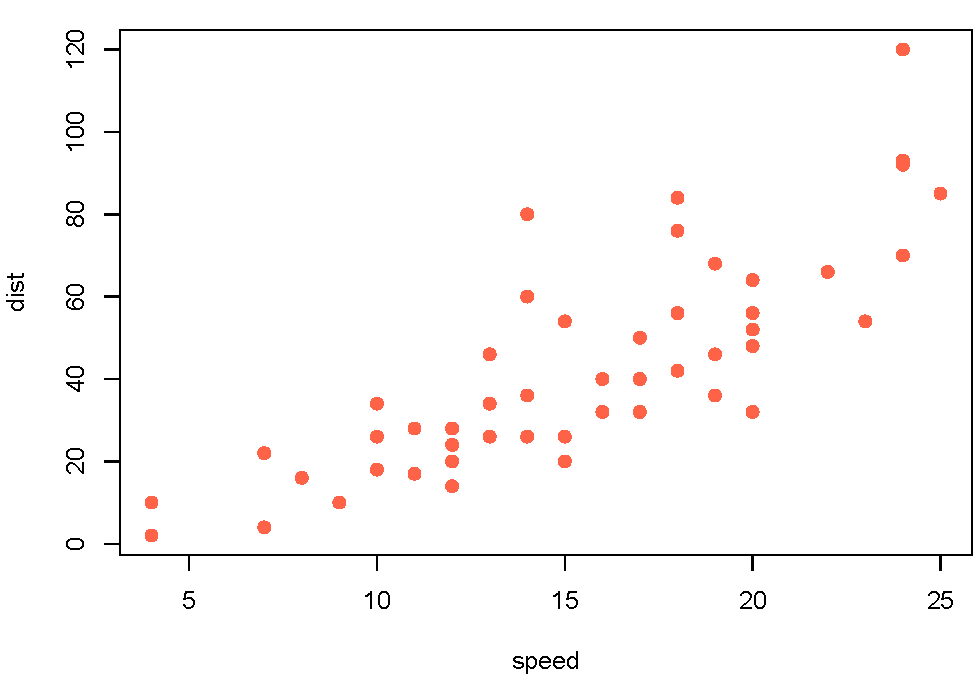
\includegraphics[width=0.9\linewidth]{plantilla_bookdown_files/figure-latex/hello-1} \caption{Hello World!}\label{fig:hello}
\end{figure}

\begin{Shaded}
\begin{Highlighting}[]
\NormalTok{knitr}\SpecialCharTok{::}\FunctionTok{kable}\NormalTok{(}
  \FunctionTok{head}\NormalTok{(iris), }\AttributeTok{caption =} \StringTok{\textquotesingle{}The boring iris data.\textquotesingle{}}\NormalTok{,}
  \AttributeTok{booktabs =} \ConstantTok{TRUE}
\NormalTok{)}
\end{Highlighting}
\end{Shaded}

\begin{table}

\caption{\label{tab:iris}The boring iris data.}
\centering
\begin{tabular}[t]{rrrrl}
\toprule
Sepal.Length & Sepal.Width & Petal.Length & Petal.Width & Species\\
\midrule
5.1 & 3.5 & 1.4 & 0.2 & setosa\\
4.9 & 3.0 & 1.4 & 0.2 & setosa\\
4.7 & 3.2 & 1.3 & 0.2 & setosa\\
4.6 & 3.1 & 1.5 & 0.2 & setosa\\
5.0 & 3.6 & 1.4 & 0.2 & setosa\\
\addlinespace
5.4 & 3.9 & 1.7 & 0.4 & setosa\\
\bottomrule
\end{tabular}
\end{table}

More chapters to come in \texttt{02-foo.Rmd}, \texttt{03-bar}.Rmd, \ldots{}

\hypertarget{ecua}{%
\chapter{Ecuaciones}\label{ecua}}

En esta capítulo se muestra como crear ecuaciones con LaTeX.

\hypertarget{ecuaciones-dentro-de-un-puxe1rrafo}{%
\section{Ecuaciones dentro de un párrafo}\label{ecuaciones-dentro-de-un-puxe1rrafo}}

Se pueden incluir ecuaciones dentro de un párrafo colocando la expresión dentro de \texttt{\$\ \$}. Por ejemplo, para escribir esta fórmula \(f(x) = x^2 + 1\) se escribe \texttt{\$f(x)\ =\ x\^{}2\ +\ 1\$}.

\hypertarget{ecuaciones-entre-puxe1rrafos}{%
\section{Ecuaciones entre párrafos}\label{ecuaciones-entre-puxe1rrafos}}

Se pueden colocar ecuaciones entre párrafos colocando la expresión de dos formas:

\begin{itemize}
\tightlist
\item
  \texttt{\$\$\ aqui\ la\ expresion\ \$\$}.
\item
  \texttt{\textbackslash{}begin\{equation\}\ aqui\ la\ expresion\ \textbackslash{}end\{equation\}}.
\end{itemize}

La siguiente expresión

\[
F = m \times a
\]

se obtuvo escribiendo

\texttt{\$\$\ F\ =\ m\ \textbackslash{}times\ a\ \$\$}

La expresión \eqref{eq:binom} siguiente

\begin{equation} 
  f\left(k\right) = \binom{n}{k} p^k\left(1-p\right)^{n-k}
  \label{eq:binom}
\end{equation}

se obtuvo escribiendo

\begin{verbatim}
\begin{equation} 
  f\left(k\right) = \binom{n}{k} p^k\left(1-p\right)^{n-k}
  \label{eq:binom}
\end{equation} 
\end{verbatim}

y para referenciarla se escribe \texttt{\textbackslash{}@ref(eq:binom)} con lo cual se obtiene la numeración \eqref{eq:binom}.

\begin{rmdtip}
Para obtener más detalles de cómo incluir ecuaciones se recomienda consultar este \href{https://bookdown.org/yihui/bookdown/markdown-extensions-by-bookdown.html\#theorems}{enlace}.
\end{rmdtip}

\hypertarget{svm}{%
\chapter{Support vector machine}\label{svm}}

\citet{Cortes1995} en el artículo titulado ``Support-Vector Networks'' propusieron las máquinas de soporte vectorial (svm) para el problema de clasificación.

Abajo se muestra una ilustración del método.

\begin{figure}

{\centering 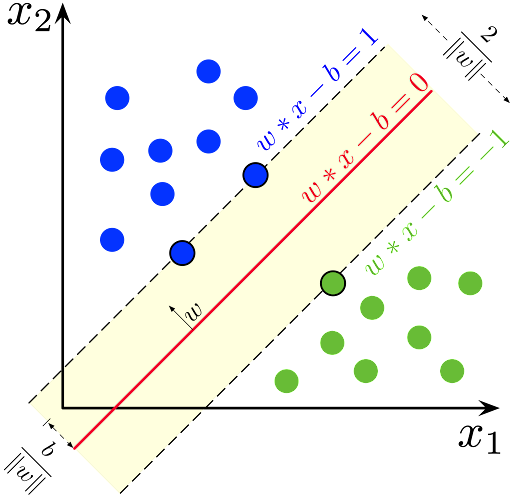
\includegraphics[width=0.6\linewidth]{images/svm} 

}

\caption{Ilustración de svm.}\label{fig:rmarkdown}
\end{figure}

\cleardoublepage

\hypertarget{appendix-appendix}{%
\appendix \addcontentsline{toc}{chapter}{\appendixname}}


\hypertarget{more-to-say}{%
\chapter{More to Say}\label{more-to-say}}

Yeah! I have finished my book, but I have more to say about some topics. Let me explain them in this appendix.

To know more about \textbf{bookdown}, see \url{https://bookdown.org}.

  \bibliography{book.bib,packages.bib}

\backmatter
\printindex

\end{document}
